%%%%%%%%%%%%%%%%%%%%%%%%%%%%%%%%%%%%%%%%%
% Beamer Presentation
% LaTeX Template
% Version 1.0 (10/11/12)
%
% This template has been downloaded from:
% http://www.LaTeXTemplates.com
%
% License:
% CC BY-NC-SA 3.0 (http://creativecommons.org/licenses/by-nc-sa/3.0/)
%
%%%%%%%%%%%%%%%%%%%%%%%%%%%%%%%%%%%%%%%%%

%----------------------------------------------------------------------------------------
%	PACKAGES AND THEMES
%----------------------------------------------------------------------------------------

\documentclass{beamer}
\mode<presentation> {

% The Beamer class comes with a number of default slide themes
% which change the colors and layouts of slides. Below this is a list
% of all the themes, uncomment each in turn to see what they look like.

%\usetheme{default}
%\usetheme{AnnArbor}
%\usetheme{Antibes}
%\usetheme{Bergen}
%\usetheme{Berkeley}
%\usetheme{Berlin}
%\usetheme{Boadilla}
%\usetheme{CambridgeUS}
%\usetheme{Copenhagen}
%\usetheme{Darmstadt}
%\usetheme{Dresden}
%\usetheme{Frankfurt}
%\usetheme{Goettingen}
%\usetheme{Hannover}
%\usetheme{Ilmenau}
%\usetheme{JuanLesPins}
%\usetheme{Luebeck}
\usetheme{Madrid}
%\usetheme{Malmoe}
%\usetheme{Marburg}
%\usetheme{Montpellier}
%\usetheme{PaloAlto}
%\usetheme{Pittsburgh}
%\usetheme{Rochester}
%\usetheme{Singapore}
%\usetheme{Szeged}
%\usetheme{Warsaw}

% As well as themes, the Beamer class has a number of color themes
% for any slide theme. Uncomment each of these in turn to see how it
% changes the colors of your current slide theme.

%\usecolortheme{albatross}
\usecolortheme{beaver}
%\usecolortheme{beetle}
%\usecolortheme{crane}
%\usecolortheme{dolphin}
%\usecolortheme{dove}
%\usecolortheme{fly}
%\usecolortheme{lily}
%\usecolortheme{orchid}
%\usecolortheme{rose}
%\usecolortheme{seagull}n
%\usecolortheme{seahorse}
%\usecolortheme{whale}
%\usecolortheme{wolverine}

%\setbeamertemplate{footline} % To remove the footer line in all slides uncomment this line
%\setbeamertemplate{footline}[page number] % To replace the footer line in all slides with a simple slide count uncomment this line

%\setbeamertemplate{navigation symbols}{} % To remove the navigation symbols from the bottom of all slides uncomment this line
}
\usepackage{color, colortbl}
\usepackage{graphicx} % Allows including images
\usepackage{booktabs} % Allows the use of \toprule, \midrule and \bottomrule in tables

\usepackage{caption}
\usepackage{subcaption}
\usepackage{float}


%\usepackage[skip=0cm,list=true,labelfont=it]{subcaption}

%----------------------------------------------------------------------------------------
%	TITLE PAGE
%----------------------------------------------------------------------------------------

\title[Fast SVDD]{Fast Support Vector Data Descriptions for Novelty Detection} % The short title appears at the bottom of every slide, the full title is only on the title page
\author[CS6011]{Aravind Sankar, CS11B033 \newline Adit Krishnan, CS11B063 \newline}

\institute[IIT Madras] % Your institution as it will appear on the bottom of every slide, may be shorthand to save space
{
IIT Madras \\ % Your institution for the title page
%\medskip
 % Your email address
}

\date{\today} % Date, can be changed to a custom date


\begin{document}
\begin{frame}
\titlepage % Print the title page as the first slide
\begin{center}
Kernel Methods for Pattern Analysis - CS6011
\end{center}
\end{frame}


%----------------------------------------------------------------------------------------

\begin{frame}
\frametitle{Introduction}
\begin{itemize}
\item We address the problem of Novelty detection, which is to detect outliers.
\item Only target class points for training - hence one class classification.
\item SVDD is one of the most popular techniques used to solve this problem.
\item SVDD constructs a soft minimal hypersphere around target class points in KFS.
\item Testing complexity of SVDD is $O(N_s)$ where $N_s$ is the number of support vectors. \\[5pt]
\end{itemize}

\textbf{Can we reduce this ?}
\end{frame}



%----------------------------------------------------------------------------------------

\begin{frame}
\frametitle{Background - SVDD}
The SVDD problem is formulated as :


\begin{equation}
\begin{split}
\text{min} \; R^2 + C \sum\limits_{i=1}^N \xi_i \\
\text{subject to}\\
||\phi(x_i) - a_{\phi}||^2  \leq R^2 + \xi_i \\
\xi_i \geq 0 \;\; \forall i = 1,...N
\end{split}
\end{equation}


\textbf{Discriminant function (assuming normalized kernel) : }

\[ g(x)  =  c - 2 \sum\limits_{i=1}^{N_s}\alpha_i K(x,x_i)\]

\end{frame}

%----------------------------------------------------------------------------------------


\begin{frame}
\frametitle{Pre-image of center (1)}

If we can find the pre-image of the center, then $N_s$ computations are not needed. 
It can be shown that the center $a_\phi$ must lie inside the unit hypersphere centered at $O_\phi$.  \\[5pt]

The sphere center $a_\phi$ is given by :
\begin{equation}
\begin{split}
a_\phi  &= \sum\limits_{i=1}^{N_s} \alpha_i \phi(x_i)  \\ 
|| \sum\limits_{i=1}^N \alpha_i \phi(x_i) ||  &< \sum\limits_{i=1}^N || \alpha_i \phi(x_i) ||
\end{split}
\end{equation}

The LHS involves the inner products $<\phi(x_i) \phi(x_j)>$, while the RHS involves the corresponding products  $|| \phi(x_i)|| \; || \phi(x_j) ||$.

\end{frame}

%----------------------------------------------------------------------------------------



\begin{frame}
\frametitle{Pre-image of center (2)}
We know from Cauchy Schwartz inequality that, 

\[ <a,b> \leq ||a|| \; ||b|| \] 


The equality in (2) holds only if  $ \forall i \;  \forall j  \; \phi(x_i) = \phi(x_j)$.

Thus, we get 
\begin{equation}
\begin{split}
|| a_\phi || &< \sum\limits_{i=1}^N || \alpha_i \phi(x_i) ||  \\
& = \sum\limits_{i=1}^N \alpha_i ||  \phi(x_i) || \\
& =  \sum\limits_{i=1}^N \alpha_i \\
\text{Thus, } ||a_\phi|| & < 1
\end{split}
\end{equation}
\begin{center}So, preimage of $a_\phi$ does not exist in x-space.\end{center}

\end{frame}


\begin{frame}
\frametitle{Agent of the center}
\textbf{Idea of FSVDD :} Express the center $a_\phi$ in terms of a point $\psi_a$ (agent of the center) whose pre-image exists is the x-space.


\begin{figure}
\centering
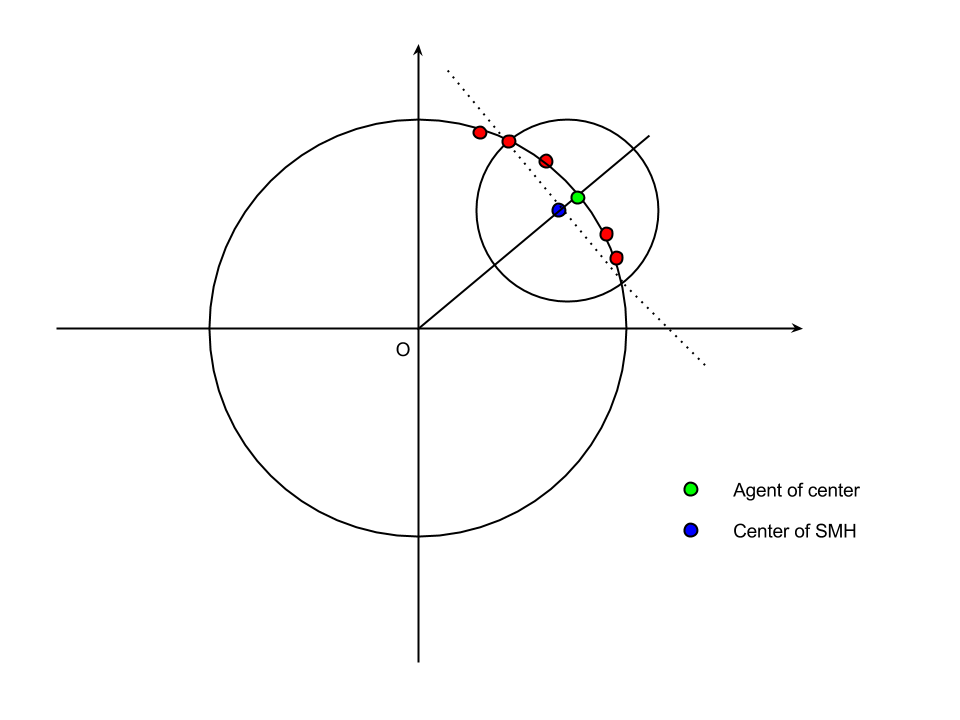
\includegraphics[width=0.9\linewidth]{SMH.png}
\caption{Caption}
\label{fig:my_label}
\end{figure}

\end{frame}

%----------------------------------------------------------------------------------------

\begin{frame}
\frametitle{Preimage of the agent (1)}
The preimage of the agent $\hat{x}$ is found by solving the problem :
\begin{equation}
\begin{split}
\hat{x} &= \; \min_{\hat{x}} ||\Psi_a - \phi(\hat{x}) ||^2  \\ 
&= \min_{\hat{x}} \; || \gamma a_\phi - \phi(\hat{x}) ||^2 \\
&= \min_{\hat{x}} \;  2 - 2 \gamma  \sum\limits_{i=1}^{N_s} \alpha_i \phi(x_i)\\
&= \min_{\hat{x}} \;  - \sum\limits_{i=1}^{N_s} \alpha_i \phi(x_i)\\
&= \min_{\hat{x}} \; \alpha^T K \alpha - 2  \sum\limits_{i=1}^{N_s} \alpha_i \phi(x_i) +1\\
&= \min_{\hat{x}} \; || a_\phi - \phi(\hat{x}) ||^2 \\
\end{split}
\end{equation}
\end{frame}


\begin{frame}
\frametitle{Preimage of the agent (2)}
On equating the derivative to 0,

\begin{equation}
\hat{x} = \frac{\sum\limits_{i=1}^N \alpha_i K(\hat{x},x_i)x_i}{\sum\limits_{i=1}^N K(\hat{x},x_i)}
\end{equation}  


Two methods to solve for the optimal $\hat{x}$ :

\begin{itemize}
\item Direct (non-iterative) method - F-SVDD-1

\item Fixed point iteration  - F-SVDD-2

\end{itemize}
\end{frame}

%----------------------------------------------------------------------------------------

\begin{frame}
\frametitle{Direct method (1)}
Let us denote the preimage of $\psi_a$ as $\hat{x}$, i.e. $ \psi_a = \phi(\hat{x})$.
\[ || \phi(\hat{x}) - \phi(x_i) ||^2  = 2 - 2 K(\hat{x},x_i)  \text{ for any } x_i \in \mathbb{R}^d\] 

This can also be computed as :
\[ || \phi(\hat{x}) - \phi(x_i) ||^2  = || \gamma a_\phi - \phi(x_i) ||^2  = 2 - 2 \gamma \sum\limits_{j=1}^N K(x_i,x_j) \]

Equating the above, we get :

\[ K(\hat{x},x_i)  = \gamma \sum\limits_{j=1}^N \alpha_j K(x_j,x_i) \] 

\end{frame}

%----------------------------------------------------------------------------------------
\begin{frame}
\frametitle{Direct method (2)}

On using this in (5), we get 

\[ \hat{x} = \frac{\sum\limits_{i=1}^N \sum\limits_{j=1}^N \alpha_i \alpha_j K(x_i,x_j) x_i}{\sum\limits_{i=1}^N \sum\limits_{j=1}^N \alpha_i \alpha_j K(x_i,x_j)} \]


\end{frame}

\begin{frame}
\frametitle{Comparision with spherical methods}
While this method leads to a spherical decision boundary in the original space, How does it compare to the other methods that attempt to do this directly rather than by using the gaussian space to do it?
\\[10pt]
First let us look at the expression for the radius in the x-space.
\\[10pt]
$D_{f}$(x) = $||\phi(x) - \psi_{a}||$ - $R^{2}$
Simplifying this gives us the surface in the x space. It is a function of $\sigma$ as well as C.
\\[5pt]
On the other hand if we use a simple polynomial kernel of degree 1 and perform SVDD, we get R = $||$UBSV - $\Sigma\beta_{i}x_{i}$ $||$
\end{frame}





\begin{frame}
\frametitle{Comparision with spherical methods}
An alternate method is to build a mean centered sphere which can be used as the SMH. 
That uses the sphere $||x - \mu_{D}||$ = $R^{2}$ as the discriminant.
\\[10pt]
\begin{itemize}
\item Position - It is easy to verify that the spheres of the different methods are centered at different places. One at mean, One at $\hat{x}$ and one at $\Sigma\beta_{i}x_{i}$. \\
\item Size - R for F-SVDD depends on C and $\sigma$, for polynomial SVDD it depends only on C, for mean it depends on tuning.
\item Computational Complexity - Testing time for all 3 cases is of constant order, irrespective of dataset size.
\end{itemize}
\end{frame}





\begin{frame}
\frametitle{Experimental setup}
We compared the performance of C-SVDD, F-SVDD-1 and F-SVDD-2 on three datasets. \\[5pt]

\textbf{Datasets :}
\begin{enumerate}
\item Overlapping classes - 2 dimensions.
\item Fisher Iris dataset - 4 dimensions.
\item Wine recognition dataset - 13 dimensions.
\end{enumerate}

We also implemented a non-kernel method, which is the Artificial neural network.

Performance is measured in terms of the average error rate (TAER) and running time.

\[ \texttt{TAER} = \frac{\texttt{Number of misclassified points}}{\texttt{Total number of points}} \]


\end{frame}



%----------------------------------------------------------------------------------------
\begin{frame}
\frametitle{Overlapping Dataset Plot}
\begin{center}
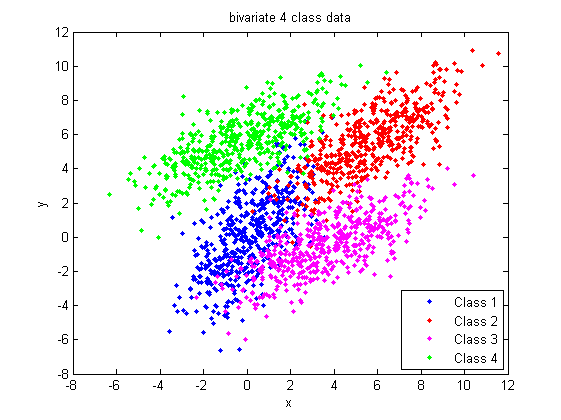
\includegraphics[scale=0.6]{data_overlapping}
\end{center}
\end{frame}


\begin{frame}
\frametitle{Example decision surface on overlapping classes dataset}

\begin{figure}[H]
\begin{subfigure}{.5\textwidth}
  \centering
  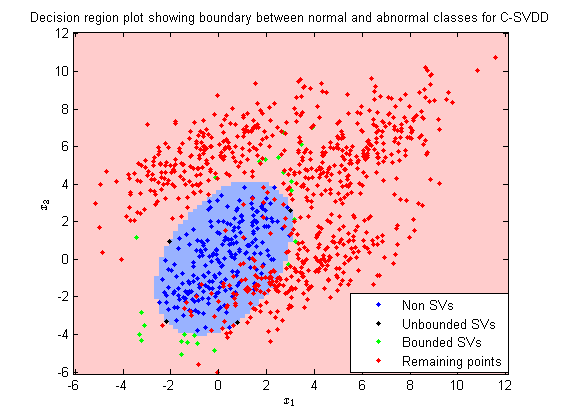
\includegraphics[width=\linewidth]{decn_over_1}
\caption{C-SVDD} 
\end{subfigure}%
\begin{subfigure}{.5\textwidth}
  \centering
  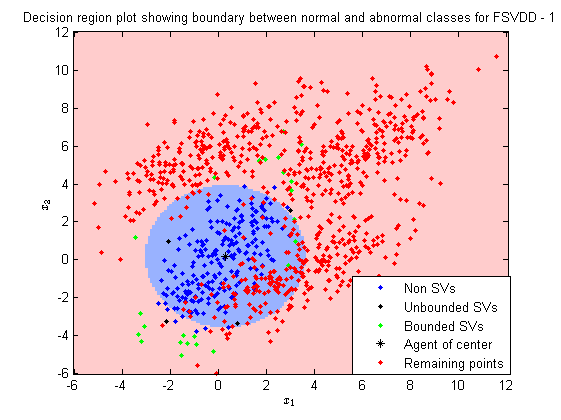
\includegraphics[width=\linewidth]{decn_over_2}
\caption{F-SVDD} 
\end{subfigure}
\caption{Decision surface - class 1 as target class} 
\end{figure}




\end{frame}

%----------------------------------------------------------------------------------------

\begin{frame}
\frametitle{Fisher Iris dataset}
\begin{figure}[H]
\begin{subfigure}{.5\textwidth}
  \centering
  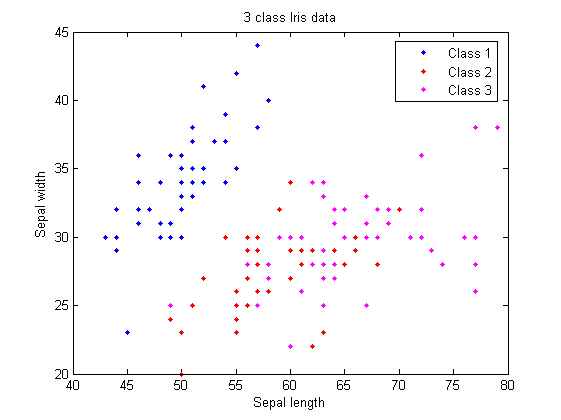
\includegraphics[width=\linewidth]{iris_1}
\caption{Scatter plot w.r.t Sepal width and length} 
\end{subfigure}%
\begin{subfigure}{.5\textwidth}
  \centering
  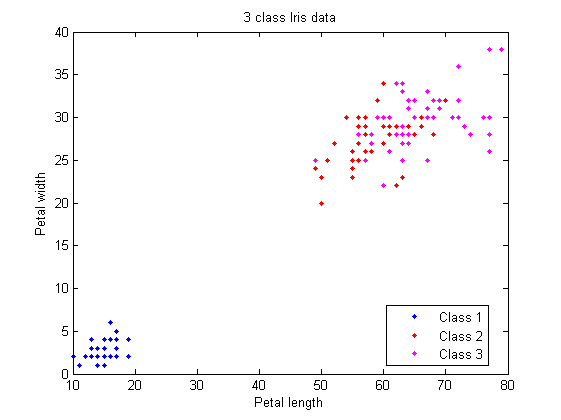
\includegraphics[width=\linewidth]{iris_2}
\caption{Scatter plot w.r.t Petal width and length} 
\end{subfigure}
\caption{Scatter plot of Fisher Iris Dataset} 
\end{figure}
\end{frame}

%----------------------------------------------------------------------------------------

\begin{frame}
\frametitle{Results on Fisher Iris dataset (1)}
\begin{table}[H]
\begin{center}
\caption{Comparison of Average Error rates on Fisher dataset}
\begin{tabular}{|c|c|c|c|c|}
\hline
Target class & C-SVDD & F-SVDD-1 & F-SVDD-2 & MLFFNN \\ \hline
1 ($N_{train} = 25$) &  0.0224  & 0.0275  & 0.0296  & 0.0105 \\ \hline
2 ($N_{train} = 25$) &  0.0632  &  0.0780  & 0.0864  & 0.1492 \\ \hline
3 ($N_{train} = 25$) & 0.0616  &  0.0884  & 0.0832 & 0.0800 \\ \hline
Average TAER &  0.0491 & 0.0646 &  0.0664 & 0.0799\\ \hline
\end{tabular}
\end{center}
\end{table}

\begin{itemize}
\item The error rates for class 2 and 3 are higher than that of class 1. This is because points
of class 1 are separable while classes 2 and 3 overlap.
\item  Difference in average TAER with C-SVDD is only 1.5 \%
\end{itemize}
\end{frame}



\begin{frame}
\frametitle{Results on Fisher Iris dataset (2)}
The observed running times on this dataset for the different algorithms are shown below :

\begin{table}[H]
\begin{center}
\caption{Running time comparison for Fisher Iris dataset}
\begin{tabular}{|c|c|c|c|c|c|c|}
\hline
Class & \multicolumn{2}{|c|}{C-SVDD} & \multicolumn{2}{|c|}{F-SVDD-1} & \multicolumn{2}{|c|}{FSVDD-2}  \\ \hline
& Training & Testing & Training & Testing & Training & Testing \\ \hline
1  & 0.02028 & 0.0109 & 0.02496  & 0.0031 & 0.0468 & 0.0015 \\ \hline
2  & 0.02184 & 0.00936 & 0.0281  &  0.0015 & 0.0577 & 0.0015 \\ \hline
3  &  0.02808 &  0.01248 & 0.0218  & 0.0031 & 0.0748 & 0.0015 \\ \hline

\end{tabular} \\[5pt]
\end{center}
\end{table}

\end{frame}


\begin{frame}

\frametitle{Results on wine recognition dataset}
Class 2 in this dataset overlaps with both the other classes quite a lot.
\begin{table}[H]
\begin{center}
\caption{Comparison of Average Error rates on Wine Recognition dataset}
\begin{tabular}{|c|c|c|c|c|}
\hline
Target class & C-SVDD & F-SVDD-1 & F-SVDD-2 & MLFFNN \\ \hline
1 ($N_{train} = 29$) & 0.0464   & 0.0554  & 0.0632   & 0.0268\\ \hline
2 ($N_{train} = 35$) &  0.2052  &  0.2426   & 0.2592   & 0.2517 \\ \hline
3 ($N_{train} = 24$) & 0.0424   &  0.0482  &  0.0548 &  0.2013 \\ \hline
Average TAER &  0.0980 & 0.1154 & 0.1257 &  0.1599 \\ \hline

\end{tabular}
\end{center}
\end{table}



\end{frame}


\begin{frame}
\frametitle{Running times on Wine Dataset}
The following are the running times on the wine dataset.
\begin{center}
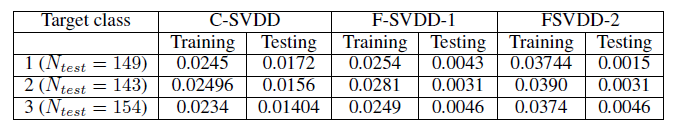
\includegraphics[scale=0.7]{wine_runtime}
\end{center}
\end{frame}

%----------------------------------------------------------------------------------------

%\begin{frame}
%\frametitle{Contents} % Table of contents slide, comment this block out to remove it
%\tableofcontents % Throughout your presentation, if you choose to use \section{} and \subsection{} commands, these will automatically be printed on this slide as an overview of your presentation
%\end{frame}

%----------------------------------------------------------------------------------------
%	PRESENTATION SLIDES
%----------------------------------------------------------------------------------------
%\section{Introduction}





\begin{frame}
\frametitle{Comparison (1)}
F-SVDD gives rise to spherical decision boundaries in the x-space, if gaussian kernel is used. 
The discriminant function reduces to :

\[ || x - \hat{x}||^2 = 2 \sigma^2 (1 - \log{\gamma c'}) = c''\] 

This may not be sufficient to separate the 2 classes. Consider the 2-Ellipses dataset below :



\begin{figure}
\centering
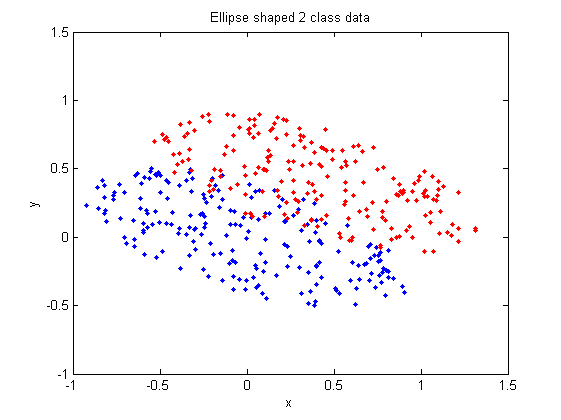
\includegraphics[scale=0.45]{data.png}
\caption{Caption}
\end{figure}




\end{frame}
%----------------------------------------------------------------------------------------

\begin{frame}
\frametitle{Comparison (2)}

\begin{figure}[H]
\begin{subfigure}{.5\textwidth}
  \centering
  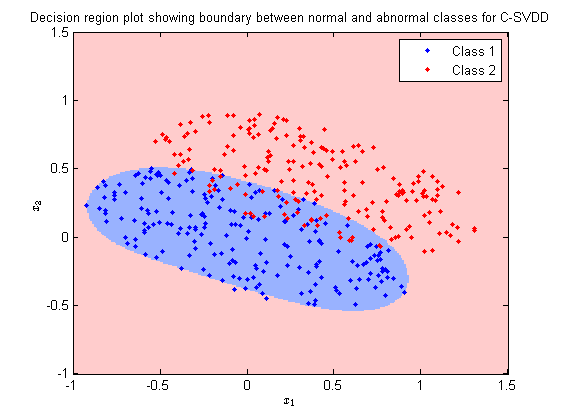
\includegraphics[width=\linewidth]{decn1}
\caption{C-SVDD} 
\end{subfigure}%
\begin{subfigure}{.5\textwidth}
  \centering
  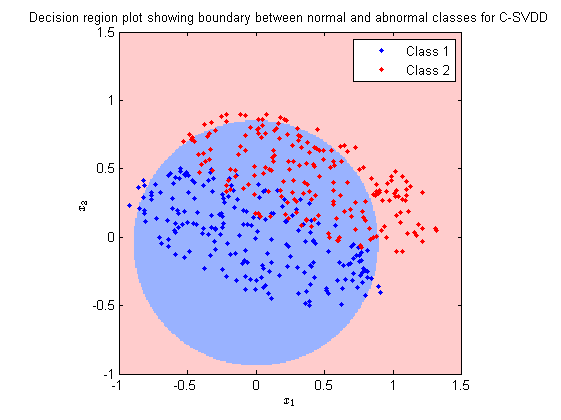
\includegraphics[width=\linewidth]{decn2}
\caption{F-SVDD} 
\end{subfigure}
\caption{Decision region plot} 
\end{figure}


\end{frame}



%----------------------------------------------------------------------------------------


\begin{frame}
\frametitle{Conclusion}
\begin{itemize}
\item F-SVDD proves to be a very efficient algorithm.
\item Reduction in space complexity, as support vectors need not be stored.
\item Suitable for real-time novelty detection systems where speed is of primary importance.
\item There is a small dip in classification performance in comparison to C-SVDD.
\item Requires the use of a normalized kernel, such as gaussian. Could lead to simple decision surfaces in the x-space.

\end{itemize}
\end{frame}


\end{document}